\chapter{Fundamentação Teórica}
\label{chap:fundteor}

\begin{flushright}

   \begin{list}{}{
      \setlength{\leftmargin}{4.5cm}
      \setlength{\rightmargin}{0cm}
      \setlength{\labelwidth}{0pt}
      \setlength{\labelsep}{\leftmargin}}
      \item Quanto maior for a rapidez de transformação de uma
      sociedade, mais temporárias são as necessidades
      individuais. Essas flutuaçõess tornam ainda mais acelerado
      o senso de turbilh da sociedade.

      \begin{list}{}{
      \setlength{\leftmargin}{0cm}
      \setlength{\rightmargin}{0cm}
      \setlength{\labelwidth}{0pt}
      \setlength{\labelsep}{\leftmargin}}
      \item (Alvin Toffler)
      \end{list}
   \end{list}
\end{flushright}

\begin{flushright}
  Quanto maior for a rapidez de transformação de uma \\
  sociedade, mais temporárias são as necessidades \\
  individuais. Essas flutuações tornam ainda mais \\
  acelerado o senso de turbilhão da sociedade. \\
  \ \\
  (Alvin Toffler)
\end{flushright}

%--------- NEW SECTION ----------------------
\section{Micromouse}
\label{sec:Micromouse}


%--------- NEW SECTION ----------------------
\section{Robotics Frameworks}
\label{sec:robotic_frameworks}



%--------- NEW SECTION ----------------------
\section{Estudo do estado da arte}
\label{sec:sota}
 \hspace{0.5cm} A competição Micromouse é um concurso anual na qual estudantes do mundo todo desenvolvem pequenos robôs autônomos, denominados \textit{micromouse}, postos a correr dentro de um labirinto. Dessa forma, o \textit{micromouse} que mais rápido chegar ao seu centro é o vencedor da competição.

 \begin{figure}[H]
 	\centering
 	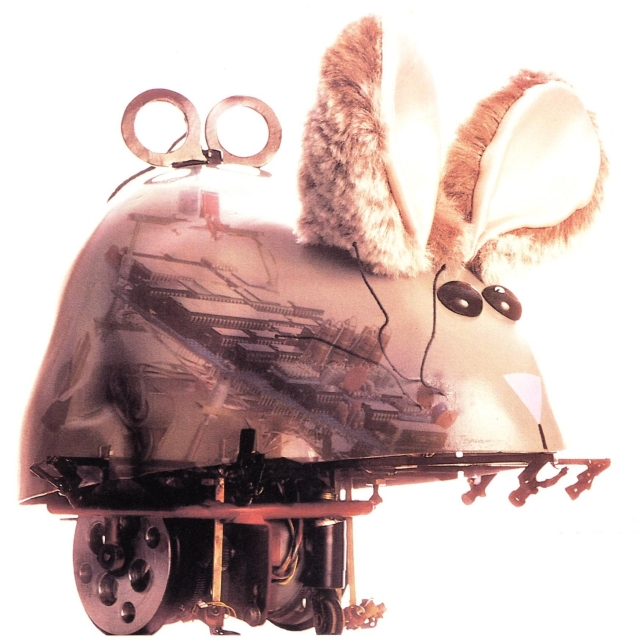
\includegraphics[width=0.5\textwidth]
 	{Figures/MoonlightSpecial.jpg}
 	\caption{\label{fig:MoonlightSpecial} Moonlight Special - Primeiro modelo \textit{micromouse} a ganhar uma competição.}
 \end{figure}

 \hspace{0.5cm} Sua ideia surge em 1977, quando a \textit{IEEE Spectrum Magazine} trouxe pela primeira vez o conceito de robôs autônomos para resolução de labirintos. Pouco tempo depois, sua primeira competição foi realizada, em junho de 1979, na primeira \textit{IEEE Amazing Micromouse Maze Contest} organizada na cidade de Nova York. Rapidamente, o conceito da competição se espalhou e, já no começo da década de 90, vários clubes voltados para Micromouse surgiam em escolas e universidades do mundo todo.\textbf{[From: The inception of Chedda] }
 
 \hspace{0.5cm} Atualmente, a \textit{IEEE Micromouse Competition} adota uma configuração que consiste-se de um labirinto de 16 x 16 blocos. Cada bloco possui 18 cm x 18 cm. As paredes, que possuem 5 cm de altura, são pintadas de branco de modo a ser reflexiva à luz infravermelho. O chão, por outro lado, é pintado de preto, para que não seja reflexivo. Além disso, o \textit{micromouse} sempre inicia a partir de um dos cantos do labirintos e termina em seu centro. Com base nisso, os competidores devem usar de algoritimos de busca para explorar o labirinto para encontrar a rota mais otimizada para a resolução do labirinto. O robô por sua vez, não pode ter suas dimensões maiores que uma seção de 25cm x 25 cm. As regras completas estão dispostas como anexo no final do documento.


%--------- NEW SECTION ----------------------
\section{Benchmark}
\label{sec:benchmark}

\subsection{GreenGiant}
\hspace{0.5cm} A Green Giant é uma desenvolvedora de múltiplas plataformas de robótica, especializada em eletrônica embarcada, tendo como seu carro-chefe o \textit{micromouse}. Seu modelo mais recente, 2016 - 2017, é voltado para alto desempenho em competições, alcançando a posição de quarto lugar durante a APEC de 2016. Sua interface de usuário possui display LED, sinalizadores luminosos de led, butões, buzzer, além de possuir um sistema de comunicação Bluetooth 4.0. Ademais, o modelo usa um sistema de ventoinhas de sucção para aumentar o nível de aderência das rodas, permitindo alcançar maiores velocidades sem derrapar.

\begin{figure}[H]
	\centering
	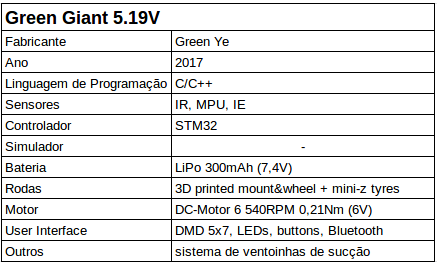
\includegraphics[width=0.7\textwidth]
	{Figures/GreenGiant.png}
	\caption{\label{fig:Green_Giant} Green Giant. }
\end{figure}


\textbf{Pontos Positivos:}
\begin{itemize}
	\item Produto de alto desempenho em competições;
	\item Sistema de ventoinhas de sucção; 
\end{itemize}


\textbf{Pontos Negativos:}
\begin{itemize}
	\item Não possui suporte à simulação;
	\item Projeto pouco documentado;
	\item Não possui guia para usuário;
	\item Não possui suporte nativo para ambiente ROS;
\end{itemize}


\subsection{WPISmartMouse}
\hspace{0.5cm} A organização estudantil, WPI CollabLab, compartilham um espaço de laboratório entre seus membros para projetos com viez colaborativo com a sociedade. Nesse espaço desenvolveu-se o Smartmouse, projeto \textit{micromouse} voltado para a competição Micromouse \textit{Brown IEEE Robotic} Olympiad. O projeto também se extendeu para o desenvolvimento de um ambiente de simulação apartir dos projetos Gazebo e Ignition, não possuindo entretanto suporte para ROS.

\begin{figure}[H]
	\centering
	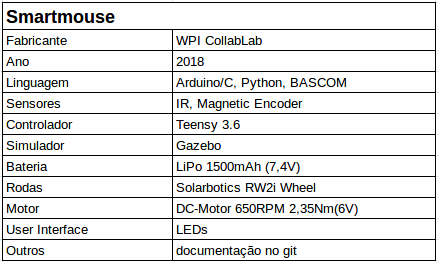
\includegraphics[width=0.7\textwidth]
	{Figures/WPISmartMouse.png}
	\caption{\label{fig:WPISmartMouse} WPISmartMouse. }
\end{figure}

\textbf{Pontos Positivos:}
\begin{itemize}
	\item Prover ferramenta de simulação;
	\item Documentação disponível no gitub;
	\item Possui portabilidade para mais de uma linguagem de programação; 
\end{itemize}

\textbf{Pontos Negativos:}
\begin{itemize}
	\item Não possui suporte nativo para ambiente ROS;
	\item Pouca variedade de sensores;
	\item Não possui guia para usuário;
	\item Poucos recursos na interface com o usuário;
\end{itemize}

%--------- NEW SECTION ----------------------
\section{Assunto 2}
\label{sec:ass2}
flkjasdlkfjasdlkfjs

